\chapter{Proposed Approach}
Our work commenced with an analysis of the paper by Kolykhalova et al. \cite{kolykhalova:2020} and its subsequent implementation in the publication by Matthiopoulou et al. \cite{inproceedings_matteopropoli}, 
retaining some aspects of the previous research while introducing a different and more comprehensive approach for predicting movement origins using machine learning.\\

We developed for visualization purposes a method to prevent inconsistent coloring behaviours among clusters over time, by introducing a novel cluster stabilization algorithm.\\
This can aid in visualization to identify any potential origins of movement.\\

Another improvement made was to retrieve and expand the previous dataset using movement fragments. 
We chose to utilize a subset of the previous dataset, and also increase the number of samples by manually annotating videos from other internal resources provided by Casa Paganini \cite{casaPaganini}.\\ 
This choice has been motivated by the necessity to have many short samples that clearly present an origin of movement instead of few samples that are hard to infer in terms of origin of movement. 
This approach aimed to achieve high-quality data suitable for implementation in machine learning techniques for pure classification purposes.\\
\\
The step forward we bring compared to the previous work is that, starting from a robust ground truth, we explored two different types of classification algorithms.
Compared to the previous work, we will be able to perform a classification that is not mediated by the consensus of multiple participants but rather focuses on automating the process.

\paragraph{Roadmap}
From the starting point of the previous work, we re-implemented and modified the approach based on graphs and improved the whole framework introducing a novel machine learning-based pipeline.

The first part of our work was done from an algorithmic perspective to enhance the existing method.
A modification we made to the previous work was to compare two similarity measurement methods: the one implemented in the original work and Cosine Similarity (explained in Section \ref{subsec:cosine_sim}).\\
Furthermore, we simplified the Game Theory to a simple WDC to expedite the pipeline and avoid calculating $20!$ coalitions.\\
We shifted the validation of fragments to the beginning of the pipeline, using a multi-step validation mechanism between expert and non-expert annotators. 
This was done to minimize the potential effects of biases that could have been introduced into the model we would subsequently use.

The second part of our work concerns the development of a machine learning approach to achieve classification of the origin of movement, not just perceived but actual. 
We focused extensively on the dataset to attain a robust method for automatic recognition.\\

The roadmap of this thesis can be outlined as follows: \\
The manual annotation was performed through an agreement between us, two non-expert annotators, followed by an initial filtering by a third independent non-expert annotator.
Finally, the last filtering was applied by an expert performer.
So the final dataset was composed by only those samples that received consensus among all the annotators.
\\
Our work encompass the reaching of three main objectives.\\
A \textbf{Cluster Transistion Smoothing Algorithm} which ensure that clusters representing groups of related markers or joints, maintain their consistency and coherence over time.
This first one is just for visualization purposes and does not implement a classification method that can be compared with the others.\\
A \textbf{Graph-based Procedure} to recognize the Origin of Movement by identifying key nodes that play pivotal roles in the motion analysis using an algorithmic method that has been handcrafted for this dataset.\\
A \textbf{Machine Learning Model} that perform the same classification task as the previous, but automatically recognizes patterns within the data, without explicitly coding them by hand.

Considering the multifaceted objectives, two parallel pipelines were developed, with the compression procedure of the markers being the only common aspect inherited from the previous work.
\\
From now we will refer to the Figure \ref{fig:walktrough} for the steps.
The algorithmic pipeline (on the left) encompasses several more steps than the other (on the right). 
\\
Initially, we smooth the time series of each sample of movement in order to clean the data from impurities such as noise, missing data for markers occlusion or tracking errors that could end up creating unnatural accelerations of some markers (Timeseries Smoothing).

Subsequently, we extract physical derived measurements from the trajectories, like the speed, acceleration and angular momentum from the smoothed data (Features Extraction). \\
Then, employing a model of human body joints, we apply cosine similarity to connected pairs of joints (Cosine Similarity). 
This aids in clustering joints within each movement frame. \\
The primary aim at this stage is to ensure the stability of color changes within these clusters. \\
Additionally, we construct a secondary graph, where only nodes at cluster borders are interconnected (Auxiliary Graph).
These nodes are weighted based on their connections and ranked across all frames (Weighted Degree Centrality).

The machine learning pipeline (on the right) follows a different approach on the data. 
We start by normalizing the dataset concerning segment length, the performer's body structure, and the complete movement trajectory (Timeseries Normalization).\\
Following this, we extract a diverse set of pertinent features from this set of normalized timeseries (Features Extraction).\\
These extracted features are then utilized to train a machine learning model (Machine Learning Model), whose performance is thoroughly evaluated using diverse metrics (Evaluation Metrics).

Finally, the results from each pipeline are compared and contrasted to evaluate their individual effectiveness.

\clearpage
\begin{figure}[H]
    \centering
    \vspace*{\fill}
    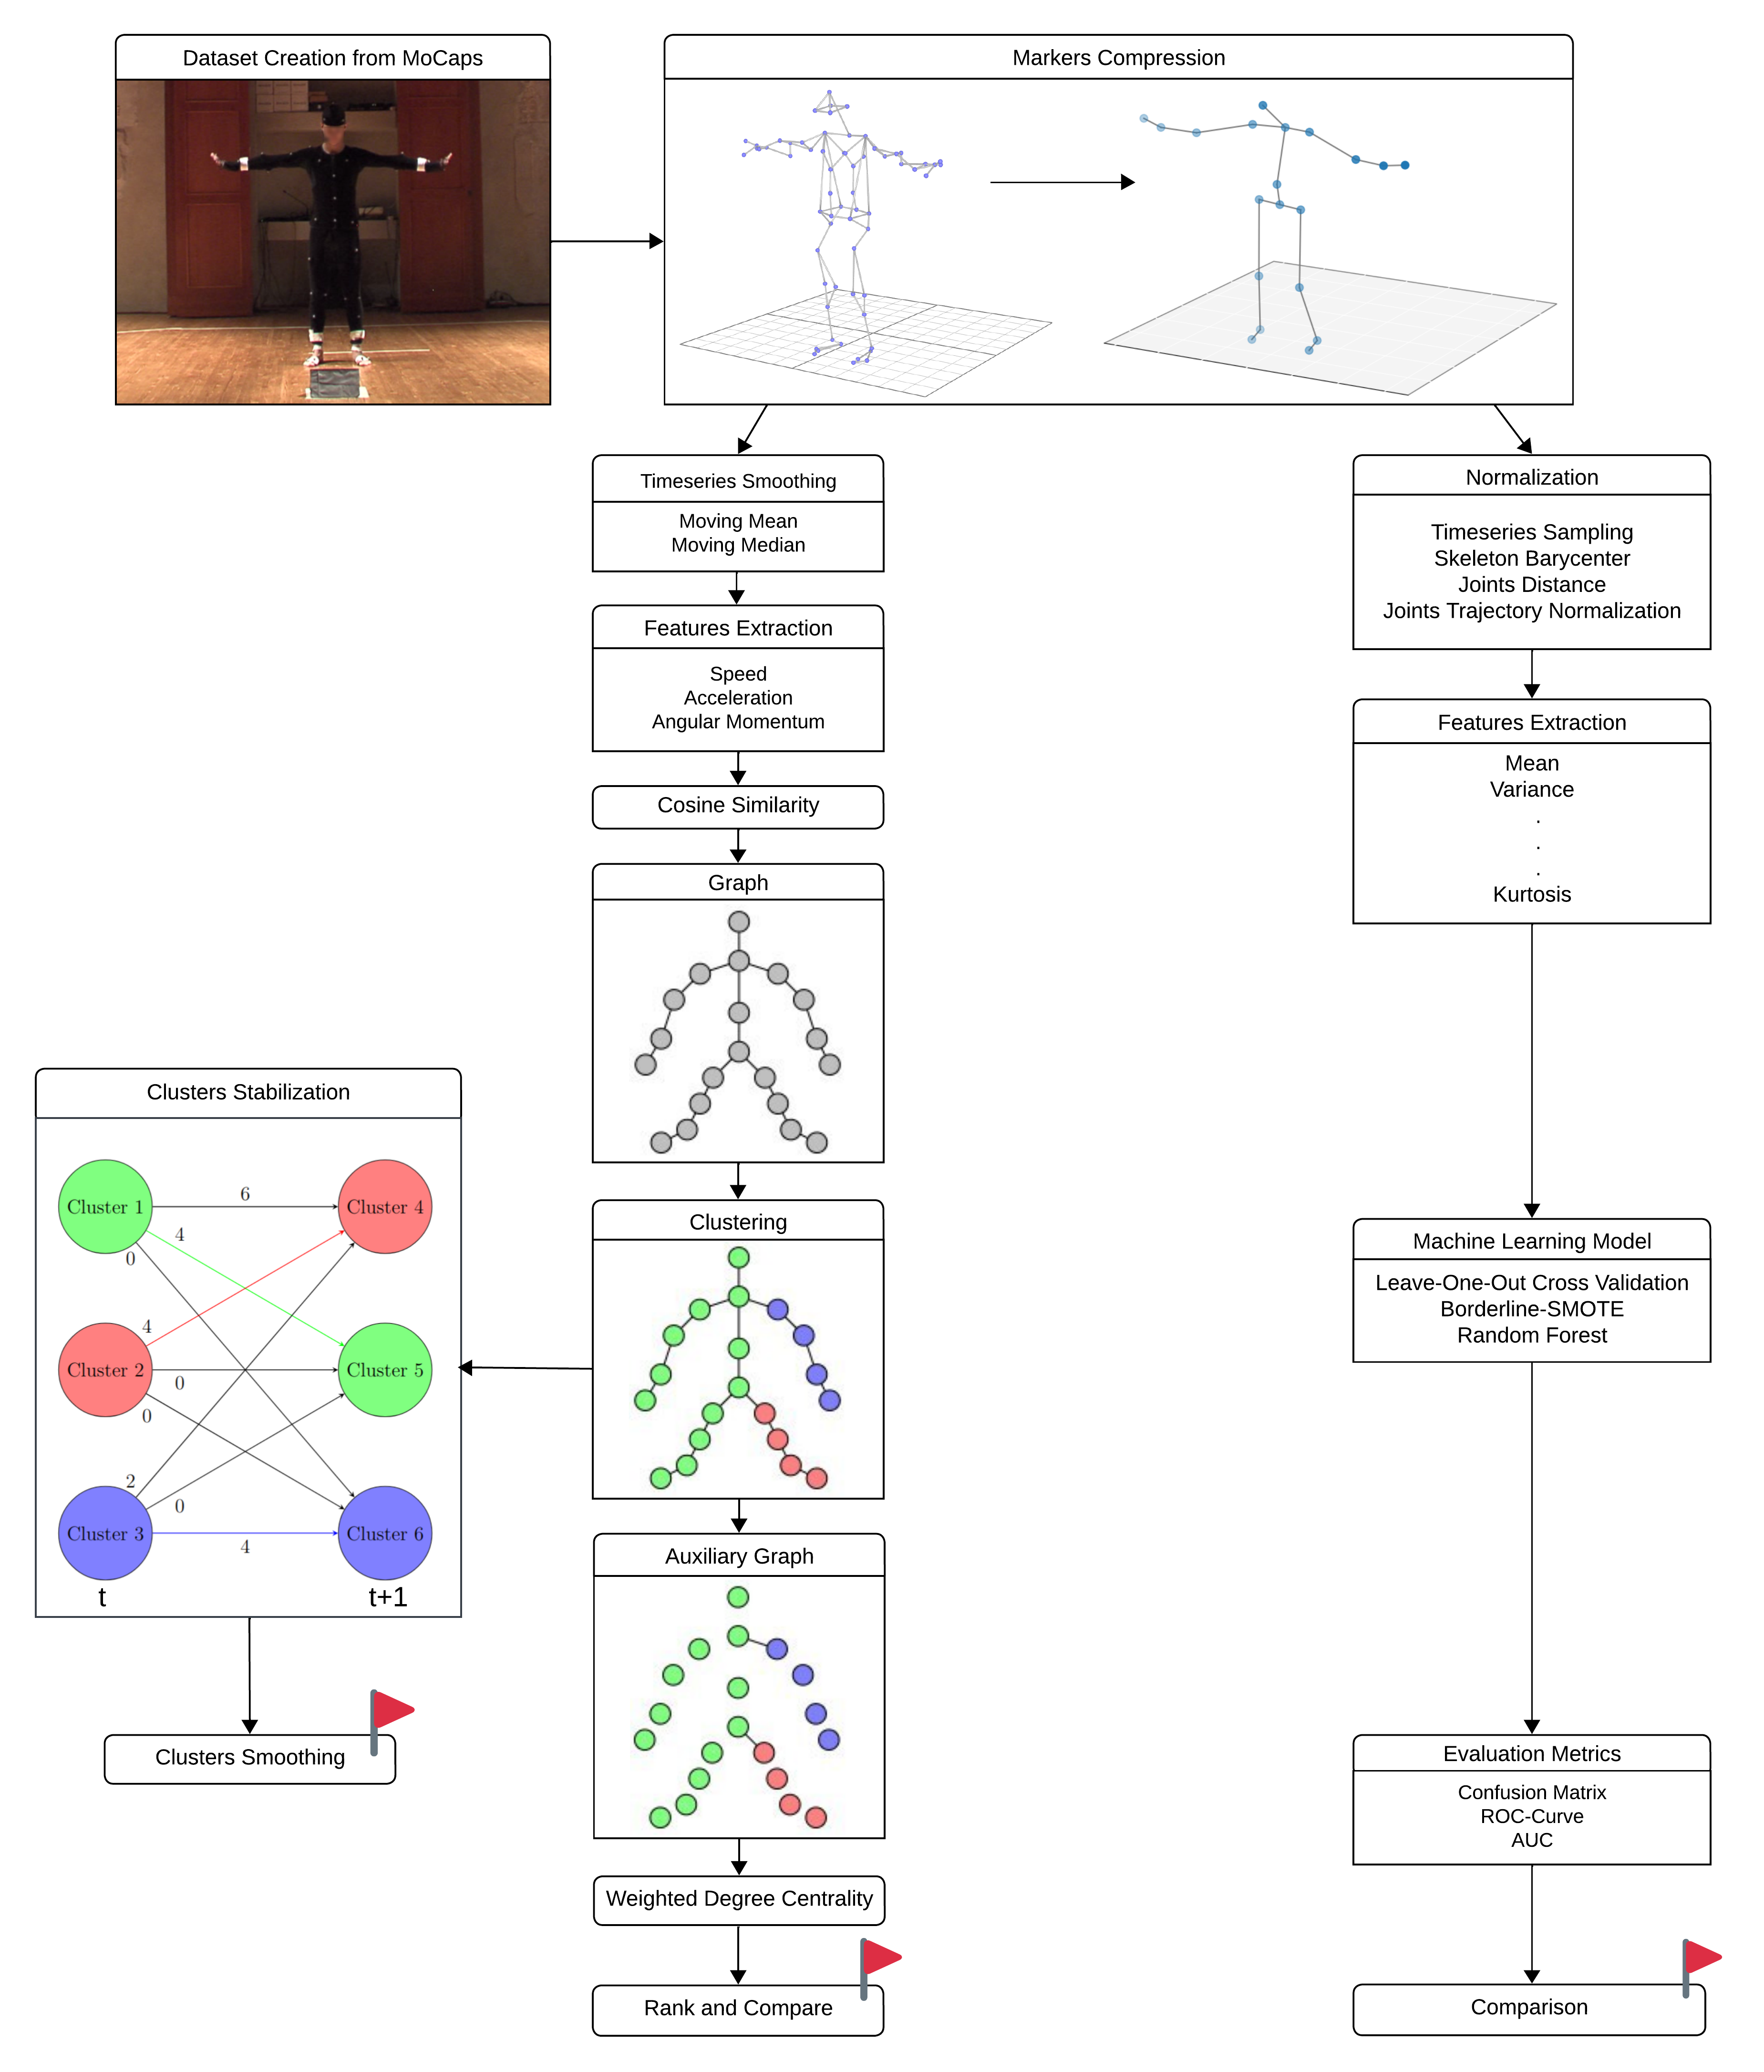
\includegraphics[width=\textwidth,height=\textheight,keepaspectratio]{Walkthrough.png}
    \caption{Roadmap of this Thesis}
    \label{fig:walktrough}
    \vspace*{\fill}
\end{figure}